\documentclass[xcolor=table,notes]{beamer}

\usepackage{pgfpages}
\usepackage[utf8]{inputenc}
\usepackage[T1]{fontenc}
\usepackage{lmodern}
\usepackage[style=ieee]{biblatex}
\usepackage{svg}
\usepackage{psfrag}
\usepackage{amsfonts}
\usepackage{supertabular}
\usepackage{array}
\usepackage{tabularx}
\usepackage{hhline}
\usepackage{minted}
\usepackage{url}
\usepackage{microtype}
\usepackage{booktabs} % for professional tables
\usepackage{makecell}
\usepackage{rotating}
\usepackage{multicol}
\usepackage{cuted}
\usepackage{colortbl}
\usepackage{adjustbox}
\usepackage{color,soul}
\usepackage{subfigure}
\usepackage{pdfpages}
\usepackage{csquotes}

\setbeamertemplate{caption}[numbered]
\setbeameroption{show notes on second screen=right}

\addbibresource[]{references.bib}

\usetheme[vertical,lang=en,pagenumbers]{NewPwr}

\title{Versioning filesystem with file history deduplication}
\subtitle{Wersjonowany system plików z deduplikacją historii zmian}
\author[author1]{Bartłomiej Chmiel}
\institute{Wydział Informatyki i Telekomunikacji}
\date{Lipiec 10, 2023}

%footcite [1]
\makeatletter
    \def\@makefnmark{\hbox{{{\usebeamercolor[fg]{footnote mark}\usebeamerfont*{footnote mark} [\@thefnmark]}}}}

    \def\@makefntext#1{%
        \def\insertfootnotetext{ #1}%
        \def\insertfootnotemark{\@makefnmark}%
        \usebeamertemplate***{footnote}}    
\makeatother


\begin{document}

	\frame{\titlepage}
	\note{
		Dzień dobry
		\\
		\\
		Pytania najlepiej na końcu
	}

	\begin{frame}{Spis treści}
		\begin{enumerate}
			\item Cel i zakres pracy
			\item Zakres pracy
			\item Przegląd wersjonowanych systemów plików
			\item Zaproponowany proces deduplikacji
			\item Otrzymane wyniki
		\end{enumerate}
		\note[item]{
			Zbadanie wpływu wykorzystania deduplikacji w wersjonowanym
			systemie plików na poprawę wydajności przestrzennej historii plików w tym systemie.
		}
		\note[item]{
			Istniejące
		wersjonowane systemy plików zostały przeanalizowane i ocenione wraz z używanymi przez nie
		strategiami deduplikacji. Na tej podstawie system plików jądra systemu Linux, NILFS, został
		wybrany jako kandydat do eksperymentalnej implementacji rozszerzenia deduplikacji postpro-
		cesowej. 
		}
		\note[item]{
			Zaprojektowane i zaimplementowane rozszerzenie zostało ocenione w porównaniu
			do podobnych rozwiązań.
		}
		\note[item]{
			Wyniki etapu ewaluacji wskazują, że deduplikacja rzeczywiście
			poprawia wydajność przestrzenną historii plików w wersjonowanym systemie plików
		}
	\end{frame}

	\begin{frame}{Cel i zakres pracy}
		\begin{itemize}
			\item Analiza metod deduplikacji historii zmian w wersjonowanych systemach plików
			\item Opracowanie i implementacja deduplikacji w wersjonowanym systemie plików
			\item Analiza porównawcza otrzymanego rozwiązania z metodami analizowanymi
					podczas przeglądu literaturowego
		\end{itemize}
	\end{frame}
	\note{
		The main goal of the thesis is to analyze the methods for file history deduplication in
		versioning filesystems and propose the implementation of file history post-process deduplication
		in a versioning filesystem. 
		\\
		\\
		The deduplication methods will be analyzed regarding their memory
		efficiency and performance. The implementation of deduplication in a versioning filesystem
		will be evaluated and compared with selected filesystems.
	}

	% \begin{frame}{Zakres pracy}
	% 	\begin{itemize}
	% 		\item Literature review and internal structure analysis of versionned filesystems.
	% 		\item Analysis of methods for change history deduplication in versionned filesystems.
	% 		\item Design and implementation of a method for change history deduplication in versionned filesystem.
	% 		\item Comparative analysis of obtained solution and methods analysed
	% 		during literature review
	% 	\end{itemize}
	% \note[item]{
	% 		Przegląd literatury i zapoznanie się z istniejącymi technologiami budowy
	% 		wersjonowanych systemów plików oraz publikacjami dotyczącymi
	% 		deduplikacji historii zmian w tychże systemach.
	% }
	% \note[item]{
	% 		Analiza rozwiązań służących deduplikacji historii zmian w
	% 		wersjonowanych systemach plików.
	% }
	% \note[item]{
	% 		Opracowanie oraz implementacja metody deduplikacji historii zmian w
	% 		wersjonowanym systemie plików.
	% }
	% \note[item]{
	% 		Analiza porównawcza otrzymanego rozwiązania z metodami analizowanymi
	% 		podczas przeglądu literaturowego
	% }
	% \end{frame}

	\begin{frame}{Przegląd wersjonowanych systemów plików}
		\begin{itemize}
			\item NILFS
			\item Btrfs
			\item CopyFS
			\item Wayback
		\end{itemize}	
	\end{frame}
	\note{
		--- Przegląd budowy tych systemów

		--- Przegląd metod deduplikacji

		--- Tylko z dostępnym kodem źródłowym

		--- Tylko reprodukowalne systemy
	}

	\begin{frame}{System plików NILFS}
		\begin{figure}
			\centering

			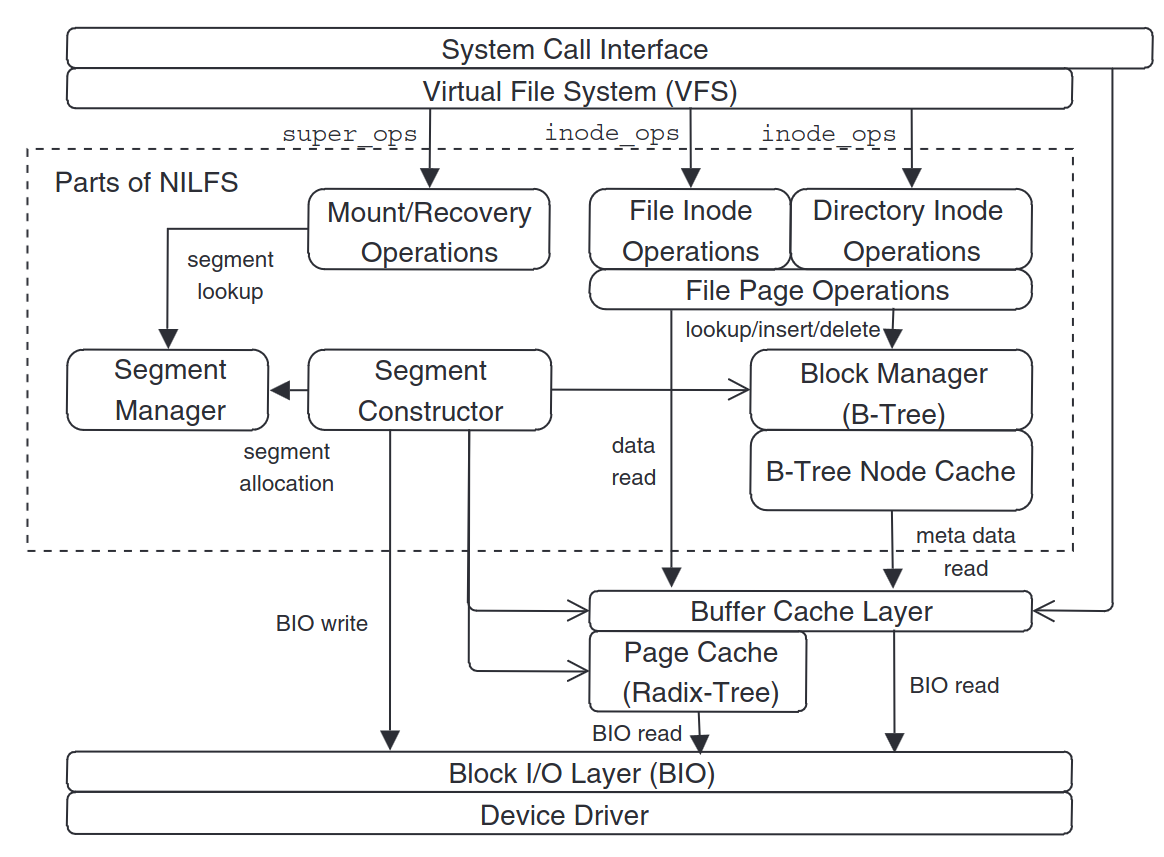
\includegraphics[width=0.9\textwidth]{media/nilfs.png}
			\caption{Struktura systemu plików NILFS w Linuxie (źródło: \cite{LinuxLogStructuredFileSystem})}
		\end{figure}	
	\end{frame}
	\note{
		Obserwacja: dzięki temu, że system używa wirtualnych bloków mapowanych na
		bloki fizyczne przez Block Manager, można sprawić, żeby do jednego fizycznego
		bloku wskazywało wiele bloków wirtualnych.
		\\
		\\
		Czemu to działa: każda modyfikacja pliku tworzy nowy
		blok w systemie (copy-on-write), więc podczas zmiany zdeduplikowanego pliku
		inny zdeduplikowany blok się nie zmieni (nie mutowalne fizyczne bloki)
		\\
		\\
		Do zapisu zmian użyć Segment Constructora
	}

	\begin{frame}{Zaproponowany proces deduplikacji}
		\begin{figure}[H]
			\centering
			\resizebox{\textwidth}{!}{%
			\includesvg{media/activity-diagram.svg}
			}
			\caption{Procesu deduplikacji (praca własna)}
		\end{figure}
	\end{frame}
	\note{
		Szybko, tylko wspomnieć o garbage collector i constructor
	}

	\begin{frame}{Implementacja}
		\begin{figure}[H]
			\centering
			\resizebox{0.8\columnwidth}{!}{%
			\includesvg{media/component-diagram.svg}
			}
			\caption{Implementacja rozszerzenia umożliwiającego deduplikację (praca własna)}
		\end{figure}
	\end{frame}
	\note{
		Szybko
		\\
		\\
		Co będzie modyfikowane?
	}

	\begin{frame}{Wyniki --- współczynnik redukcji miejsca\cite{UnderstandingDataDeduplicationRatios}}
		\begin{figure}[H]
			\centering
			\begin{equation} \label{ch2_dedup/metrics/srp}
				SRP = \frac{BD - AD}{BD}
			\end{equation}
			\begin{tabular}{@{}>{$}l<{$}l@{}}
				BD & the size of data before deduplication \\
				AD & the size of data after deduplication \\
				SRP & space reduction percentage \\
			\end{tabular}
		\end{figure}
	\end{frame}
	\note{
		Jak interpretować współczynnik?
		\\
		\\
		stosunek różnicy przed i po do tego co było przed
	}

	\begin{frame}{Wyniki --- współczynnik redukcji miejsca}
		\begin{figure}[H]
			\resizebox{0.9\columnwidth}{!}{%
			\includesvg{media/deduplication/dedup_space_reduction.svg}
			}
			\caption{Współczynnik redukcji miejsca dla deduplikacji (praca własna)}
		\end{figure}
	\end{frame}
	\note{
		Trend stały koło 5\%
		\\
		\\
		Dlaczego tak małe pliki:

		--- 16 mega to 16,777,216 bajtów czyli 4096 bloków

		--- ograniczenia środowiska testowego -> 
		tablica mieszająca (hash table) w pamięci

		--- czas wykonania 14s dla największych plików -> dużo
		operacji

		--- praca polegała na sprawdzeniu czy rzeczywiście deduplikacja
		jest możliwa, kierunki dalszego rozwóju zostały wskazane pracy 

		--- najważniejsze było sprawdzenie, że deduplikacja nie uszkadza
		plików
	}

	\begin{frame}{Wyniki --- porównanie z innymi rozwiązaniami}
		\begin{table}[H]
			\centering
			\begin{tabular}{lrrrr}
\toprule
Tool & \multicolumn{4}{r}{Space reduction percentage} \\
 & mean & min & max & std \\
\midrule
dduper & 49.57 & 44.65 & 49.90 & 0.77 \\
dedup & 4.30 & 0.44 & 25.00 & 3.08 \\
duperemove & 49.57 & 44.65 & 49.90 & 0.77 \\
\bottomrule
\end{tabular}

			\caption{Porównanie współczynników redukcji miejsca (praca własna)}
		\end{table}
	\end{frame}
	\note{
		Potwierdza trend, może być lepiej
		\\
		\\
		Odchylenie spowodowane mierzeniem deduplikacji dla bardzo
		małego systemu plików (16M)
	}

	% \begin{frame}{Results --- memory usage}
	% 	\begin{figure}[H]
	% 		\centering
	% 		\resizebox{0.9\columnwidth}{!}{%
	% 			\includesvg{media/deduplication/dedup_occupied_memory.svg}
	% 		}
	% 		\caption{Nilfs dedup memory usage (own work)}
	% 		\label{ch5_eval/dedup/memory}
	% 	\end{figure}
	% \end{frame}

	% \begin{frame}{Results --- time elapsed}
	% 	\begin{figure}[H]
	% 		\centering
	% 		\resizebox{0.9\columnwidth}{!}{%
	% 			\includesvg{media/deduplication/dedup_time_elapsed.svg}
	% 		}
	% 		\caption{Nilfs dedup time elapsed (own work)}
	% 		\label{ch5_eval/dedup/time}
	% 	\end{figure}
	% \end{frame}


	\begin{frame}[allowframebreaks]{Bibliografia}
		\printbibliography
	\end{frame}
	\note{
		Dziękuję za uwagę
	}

\end{document}
